\Exercise[number={3}]
A trained mouse lives in the house depicted in the figure, consisting of
three interconnected rooms. A bell rings at regular intervals. The mouse is
trained to move into another room as soon as the bell rings.
When the mouse changes room, it chooses at random one of the available doors.
Mouse behavior can be represented as a Markov process in which the state
specifies the room \((A, B, C)\) where the mouse is located at a given time.
Determine the state transition matrix.
\begin{figure}[H]
    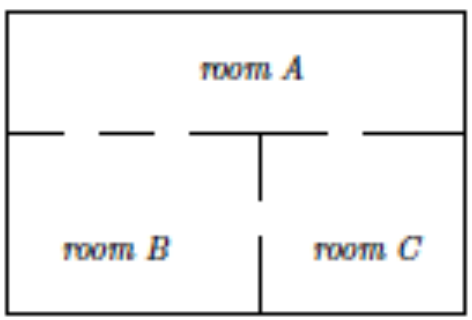
\includegraphics[scale=0.6]{E_2}
    \centering
\end{figure}

\Answer[number={3}]
The following probabilities can be obtained by simply counting the doors
available in each room, by assuming that the mouse cannot remain in the
same room for two subsequent intervals:
\begin{align*}
    \begin{matrix}
        S_{t-1}=A && S_{t-1}=B && S_{t-1}=C\\
        Pr(S_{t}=A|S_{t-1}=A)=0 && Pr(S_{t}=A|S_{t-1}=B)=\frac{2}{3} && Pr(S_{t}=A|S_{t-1}=C)=\frac{1}{2}\\
        Pr(S_{t}=B|S_{t-1}=A)=\frac{2}{3} && Pr(S_{t}=B|S_{t-1}=B)=0 && Pr(S_{t}=B|S_{t-1}=C)=\frac{1}{2}\\
        Pr(S_{t}=C|S_{t-1}=A)=\frac{1}{3} && Pr(S_{t}=C|S_{t-1}=B)=\frac{1}{3} && Pr(S_{t}=C|S_{t-1}=C)=0\\
    \end{matrix}
\end{align*}
As the state transition matrix is made of \(\phi_{ij}\) elements referred to
the \(i\)-th state \(S_{t}\) and \(j\)-th state \(S_{t-1}\), \(\Phi\) is:
\begin{align*}
    \Phi=
    \begin{bmatrix}
        \phi_{11} && \phi_{12} && \phi_{13}\\
        \phi_{21} && \phi_{22} && \phi_{23}\\
        \phi_{31} && \phi_{32} && \phi_{33}
    \end{bmatrix}
    =
    \begin{bmatrix}
        0 && \frac{2}{3} && \frac{1}{2}\\
        \frac{2}{3} && 0 && \frac{1}{2}\\
        \frac{1}{3} && \frac{1}{3} && 0
    \end{bmatrix}
\end{align*}